	\documentclass[10pt,oneside]{CBFT_book}
	% Algunos paquetes
	\usepackage{amssymb}
	\usepackage{amsmath}
	\usepackage{graphicx}
	\usepackage{libertine}
	\usepackage[bold-style=TeX]{unicode-math}
	\usepackage{lipsum}

	\usepackage{natbib}
	\setcitestyle{square}

	\usepackage{polyglossia}
	\setdefaultlanguage{spanish}
	



	\usepackage{CBFT.estilo} % Cargo la hoja de estilo

	% Tipografías
	% \setromanfont[Mapping=tex-text]{Linux Libertine O}
	% \setsansfont[Mapping=tex-text]{DejaVu Sans}
	% \setmonofont[Mapping=tex-text]{DejaVu Sans Mono}

	%===================================================================
	%	DOCUMENTO PROPIAMENTE DICHO
	%===================================================================

\begin{document}




% =================================================================================================
\chapter{Picture de interacción y perturbación dependiente del tiempo}
% =================================================================================================

Puédense escribir perturbaciones dependientes del tiempo 
\[
	H = H_0 + V(t)
\]
con $\Ket{n}$ no dependiente del tiempo. Se estudiarán transiciones entre autoestados del $H_0$ (que son 
estacionarios). Un autoestado permanece en el tiemo como tal pero con fase oscilante
\[
	\Ket{\alpha,t_0,t}_s = \euler^{-iH/\hbar(t-t_0)}\Ket{\alpha,t_0}_s
\]
\[
	= \euler^{-iH/\hbar(t-t_0)} \euler^{-iV(t)/\hbar(t-t_0)} \Ket{\alpha,t_0}
\]
\[
	= \sum_n \euler^{-iH_0/\hbar \: t} \euler^{-iV(t)/\hbar \: t} \ket{n}\Braket{n|\alpha,t_0}
\]
\[
	= \sum_n \euler^{-iE_n^0/\hbar \: t }\ket{n}\euler^{-iV(t)/\hbar \: t } \Braket{n|\alpha,t_0}	
\]
\[
	\euler^{iH_0/\hbar t}\Ket{\alpha,t_0,t}_s =
	\sum_n  \underbrace{\euler^{-iV(t)/\hbar \: t} \Braket{n|\alpha,t_0}}_{C_n(t)} \ket{n} = \Ket{\alpha,t_0,t}_I	
\]
es decir 
\[
	 \Ket{\alpha,t_0,t}_I = \euler^{iH_0/\hbar t}\Ket{\alpha,t_0,t}_s
\]
Aquí se puede pensar que 
\begin{itemize}
 \item $C_n(t)$ evoluciona por $V(t)$
 \item $\euler^{-iE_n^0 t/\hbar}$ evoluciona por $H_0$
\end{itemize}

Esto introduce la {\it picture} de interacción de Dirac; en la cual los estados evolucionan con $V(t)$.

\begin{center}
\begin{tabular}{|c|ccc|}
\hline 
& Dirac & Schrödinger & Heinsenberg \\
\hline 
% & &  & \\
estados & evolucionan & evolucionan & fijos \\
$\Ket{\alpha}$ & con $V(t)$ & con $H$ &  \\
\hline
operadores & evolucionan & fijos & evolucionan \\
 & con $H_0$ &  & con $H$ \\
\hline
base & fijos & fijos & evolucionan \\
$\Ket{a'}$ &  &  &  \\
\hline 
% & & & \\
\end{tabular}
\end{center}

\[
	i\hbar \dpar{}{t}\Ket{\alpha,t_0,t}_s = H \Ket{\alpha,t_0,t}_s
\]
\[
	i\hbar \dpar{}{t}\left( \euler^{-iH_0t/\hbar}\Ket{\alpha,t_0,t}_I \right) = 
	H \euler^{-iH_0t/\hbar} \Ket{\alpha,t_0,t}_I
\]
\[
	i\hbar \euler^{-iH_0t/\hbar}\dpar{}{t} \Ket{\alpha,t_0,t}_I = 
	V(t) \euler^{-iH_0t/\hbar} \Ket{\alpha,t_0,t}_I
\]
\[
	i\hbar \dpar{}{t} \Ket{\alpha,t_0,t}_I = V(t) \Ket{\alpha,t_0,t}_I,
\]
que es la ecuación de evolución de los kets.
Pediremos asimismo que 
\[
	_s\Braket{\; A_s \;}_s = _I\Braket{\; A_I \;}_I
\]
\[
	_I\Braket{\alpha,t_0,t|A_I|\alpha,t_0,t}_I =
	_s\Braket{\alpha,t_0,t|\euler^{-iH_0t/\hbar}A_I\euler^{iH_0t/\hbar}|\alpha,t_0,t}_s=
	_s\Braket{\alpha,t_0,t|A_s|\alpha,t_0,t}_s =
\]
Y los operadores evolucionan según 
\[
	A_I = \euler^{iH_0t/\hbar}A_s\euler^{-iH_0t/\hbar}
\]
\[
	\dtot{A_I}{t} = \frac{1}{i\hbar}[A_I, H_0]
\]
que es igual que la ecuación de Heisenberg pero con $\hat{H}_0$ en lugar de $H$.
Los kets base permanecen fijos, porque así lo hacen en Schrödinger, en realidad oscila su fase; entonces 
\[
	\Ket{n,t_0,t}_s = \euler^{-iHt/\hbar} \ket{n,t_0}_s
\]
\[
	\Ket{n,t_0,t}_I = \euler^{iH_0t/\hbar} \euler^{-iHt/\hbar} \ket{n,t_0}_s =
	\euler^{-iVt/\hbar} \ket{n,t_0}_s = \euler^{iH_0t/\hbar} \ket{n,t_0}_s
\]
\[
	\Ket{n,t_0,t}_I = \euler^{iE_0t/\hbar} \ket{n,t_0,t}_s
\]

\subsection{Evolución de los coeficientes}

\[
	\Ket{\alpha,t_0,t}_I = \sum_n \Ket{n}\Braket{n|\alpha,t_0,t}_I = \sum_n C_n(t) \Ket{n}
\]
\[
	C_n(t) = \euler^{iVt/\hbar} \Braket{n|\alpha,t_0}_s
\]
\[
	\Braket{n|\alpha,t_0,t}_I = C_m(t)
\]
con $\Ket{n},\ket{m}$ autoestados de $H_0$, le pego un $\Bra{n}$ a la ecuación de evolución de kets,
\[
	i\hbar \dpar{}{t} \Braket{n|\alpha,t_0,t}_I = \Braket{n|V_I(t)|\alpha,t_0,t}_I
\]
\[
	= \sum_m \Braket{n|V_I(t)|m}\Braket{m|\alpha,t_0,t}_I
\]
\[
	i\hbar \dpar{}{t}C_n(t) = \sum_m C_m(t) \Braket{n|V_I(t)|m}
\]
\[
	i\hbar \dpar{}{t}C_n(t) = \sum_m C_m(t) \Braket{n|V_s|m} \euler^{it(E_n-E_m)/\hbar}
\]
\[
	i\hbar \dpar{}{t}C_n(t) = \sum_m C_m(t) V_{nm}(t) \euler^{i\omega_{nm}t}
\]
donde $V_{nm}(t) \equiv \Braket{n|V(t)|m}$ y $\omega_{nm} \equiv (E_n-E_m)/\hbar$.
Esta es la ecuación que cumplen los coeficientes, donde $|C_n(t)|^2$ es la probabilidad de hallar al sistema 
en el autoestado $\Ket{n}$.
Es decir
\[
	i\hbar \begin{pmatrix}
	\dot{c}_1 \\ \dot{c}_2 \\ ... \\ \dot{c}_N \\
	\end{pmatrix} 
	=
	\begin{pmatrix}
	V_{11} & V_{12}\euler^{i\omega_{12}} & ... \\ V_{21}\euler^{i\omega_{21}} & V_{22} & ... \\ ... \\ ... \\
	\end{pmatrix}
	\begin{pmatrix}
	c_1 \\ c_2 \\ ... \\ c_N \\
	\end{pmatrix} 
\]
que puede ser de difícil solución.

\subsection{Método perturbativo (dependiente del tiempo)}

Pensaremos en una serie perturbativa 
\[
	C_n(t) = C_n(t)^{(0)} + C_n(t)^{(1)}  + C_n(t)^{(2)}  + ...
\]

El evolucionador temporal en la picture de interacción cumple 
\[
	\Ket{\alpha,t_0,t} = U_I(t,t_0)\Ket{\alpha,t_0}_I
\]
que viene de  
\[
	i\hbar \dtot{}{t} U_I(t,t_0) = V_I(t) U_I(t,t_0)
\]
con $U(t_0,t_0)=\mathbb{1}$ la cual resolviendo nos hace llegar a 
\[
	U_I(t,t_0) = \mathbb{1} - \frac{i}{\hbar}\int_{t_0}^{t} V_I(t')U_I(t',t_0) dt'
\]
y esto lleva a la serie de Dyson:
\begin{multline*}
	U_I(t,t_0) = \mathbb{1} - \frac{i}{\hbar}\int V_I(t') dt' + \left( -\frac{i}{\hbar} \right)^2\int_{t_0}^t 
	V_I(t') \int_{t_0}^{t'}V_I(t'')dt'' + ...\\ + \left( -\frac{i}{\hbar} \right)^n 
	\int_{t_0}^t dt'\int_{t_0}^{t'}dt''\int_{t_0}^{t''}dt''' ... \int_{t_0}^{t^{n-1}}dt^{n} V_I(t') 
	V_I(t'')...V_I(t^n)	
\end{multline*}



\subsection{Transiciones entre autoestados del hamiltoniano $H_0$}
\[
	\Ket{} =
\]
\[
	a
\]
La amplitud de transición será 
\[
	C
\]
con $\Ket{i},\Ket{n}$ autoestados de $H_0$.
Sea $\tilde{C}_n(t)=\Braket{n|U_s(t)|i}$ y busquemos una expresión 
\[
	a
\]
\[
	b
\]
y notemos que $\hat{U}$ no obedece la ley de transformación de operadores.

\[
	a
\]
\[
	b \Rightarrow |C_n(t)|^2 = |\tilde{C}_n(t)|^2
\]

Para transiciones entre autoestados de $H_0$ los coeficientes dan la misma probabilidad (evaluados con el 
evolucionador de Dirac que con el de Schrödinger).
Vamos a las transiciones a los tres 
\begin{itemize}
 \item orden 0
 \item orden 1
 \item orden 2
\end{itemize}

\subsection{Ejemplo: potencial constante encendido abruptamente}

Notemos que $V\neq V(t)$. Dependerá de cualquier otra cosa.
\[
	a
\]
\[
	b
\]
\begin{figure}[htb]
	\begin{center}
	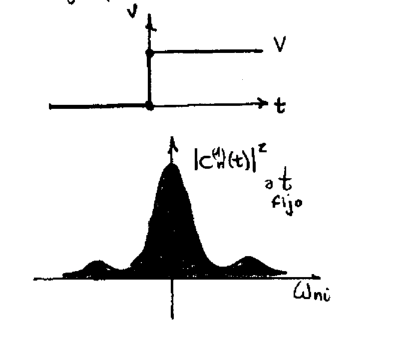
\includegraphics[width=0.6\textwidth]{images/teo2_22.pdf}
	\end{center}
	\caption{}
\end{figure} 
Es máxima la probabilidad cuando $\Delta E\to 0$. En ese caso las transiciones son a estados de la misma 
energía. A tiempo largo la probabilidad es no nula para aquellos estados 
\[
	t \sim \frac{2\pi}{|\omega_{ni}|}
\]
Hay probababilidad de transición $\Ket{i} \to \Ket{n}$ apreciable con $\Delta E \sim 0$.

\section{Scattering: orden 1}

Este último ejemplo puede aplicarse a colisiones elásticas. Prendemos y apagamos un potencial que es el 
masacote al cual impactamos. De entrada ha partículas libres y de salida (lejos de $V$) partículas libres.
Entonces $ E_n - E_c \sim 0$ y consideraremos lo que sucede a tiempos largos. Interesará la probabilidad 
total de transicionear a estados de energía similares a $E_i$. Por ello se considera 
\[
	\sum 
\]
donde el integrando es el número de estados dentro de un intervalo de energías $(E,E+dE)$.
\begin{figure}[htb]
	\begin{center}
	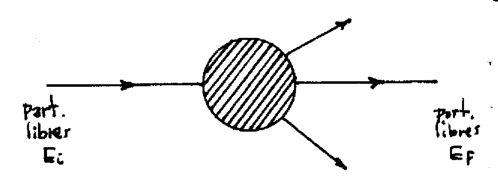
\includegraphics[width=0.6\textwidth]{images/teo2_23.pdf}
	\end{center}
	\caption{}
\end{figure} 
En tiempos muy largos la expresión [1] tiende a una delta de Dirac y se integra fácil,
\[
	\lim 
\]

La probabilidad de transición es proporcional a $t$. Se suele definir una tasa de transición (probabilidad de 
transición por unidad de tiempo)
\[
	\dtot{}{t}\left( \sum_{n(E_n\sim E_i)} |C_n^1|^2 \right) =
\]
que es la regla de oro de Fermi.

\section{El método variacional}

Se puede usar para aproximar la energía del estado fundamental (el estado de energía mínima)
\[
	=
\]
\[
	=
\]
y usamos 
\[
	\frac{|}{|} \geq E_0
\]

\subsection{Scattering a orden dos y OFPT}

Continuando con el orden dos de scattering por un $V\neq V(t)$ se tiene:
\[
	\omega
\]

Para obtener los siguientes términos dentro del $\bar{||^2}$ podemos emplear un ardid gráfico conocido como 
{\it Old Fashioned Perturbation Theory}

\begin{figure}[htb]
	\begin{center}
	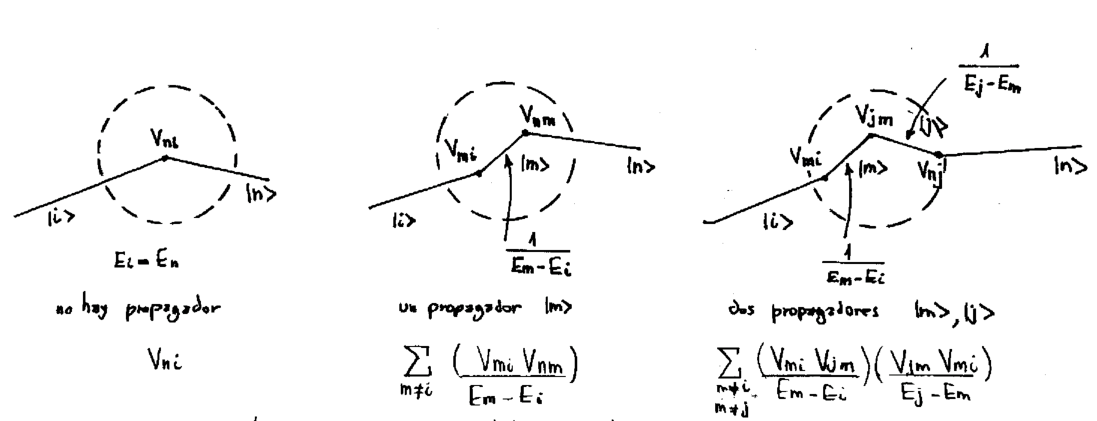
\includegraphics[width=1.0\textwidth]{images/teo2_24.pdf}
	\end{center}
	\caption{}
\end{figure} 


Fíjese que en los estados intermedios estados virtuales $\Ket{m},\Ket{j}$ no se conserva la energía. Son 
propagadores.


\subsection{Perturbación armónica}

Sea un potencial armónico y hermítico 
\[
	V(t) =
\]
quiero ver probabilidad de transición a orden uno,
\[
	C_n(t)^1 = 
\]
\[
	a
\]
\[
	b
\]
\[
	c
\]

Luego será nulo sólo si 
\[
	\omega
\]
\[
	\omega
\]

\begin{figure}[htb]
	\begin{center}
	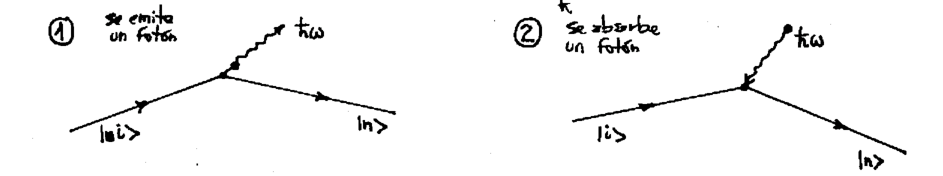
\includegraphics[width=1.0\textwidth]{images/teo2_25.pdf}
	\end{center}
	\caption{}
\end{figure} 

Luego,
\[
	\lim 
\]
representa la probababilidad de emitir o absorber fotones en una interacción. Se puede asociar que $V$ crea 
fotones y $V^\dagger$ destruye fotones. Para un átomo se tiene 
\begin{figure}[htb]
	\begin{center}
	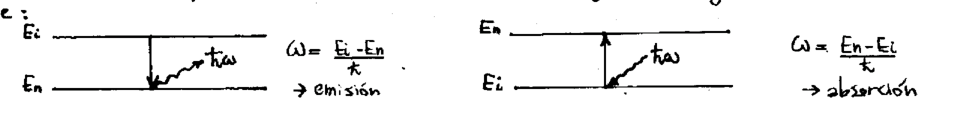
\includegraphics[width=1.0\textwidth]{images/teo2_26.pdf}
	\end{center}
	\caption{}
\end{figure} 




\section{Despoblamiento de estados iniciales}

Queremos ver con cual $v$ se despoblan los $\Ket{i}$. Para elllo me construyo un potencial {\it suave}
\[
	\lim 
\]
donde $\eta$ es un parámetro regularizador.
\begin{figure}[htb]
	\begin{center}
	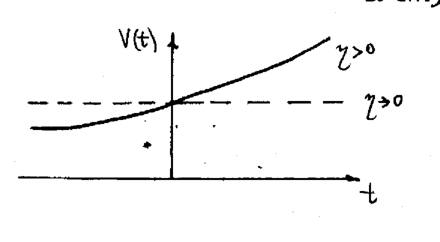
\includegraphics[width=0.6\textwidth]{images/teo2_27.pdf}
	\end{center}
	\caption{}
\end{figure} 
\[
	a
\]
\[
	b
\]
\[
 	c
\]
y tomando el límite $\eta \to 0$ 
\[
	d
\]
y llegamos a la regla de oro de Fermi,
\[
	d
\]

\subsection{Scattering sección eficaz}

$\Ket{k},\Ket{k}'$ son autoestados de momento (partículas libres),
\[
	|\vb{k}| = |\vb{k}'| 
\]
se conserva la energía. Consideraremos la aproximación más baja (aproximación de Born).
\begin{figure}[htb]
	\begin{center}
	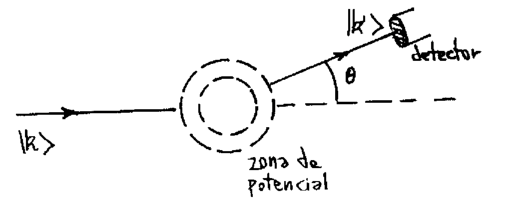
\includegraphics[width=0.6\textwidth]{images/teo2_28.pdf}
	\end{center}
	\caption{}
\end{figure} 

\[
	\omega 
\]
queremos calcular la densidad de estados de energía entre $(E,E+dE)$. Pensamos en una partícula libre en una 
caja $1D$ de longitud $L$.
\[
	N
\]
pidiendo normalización unitaria $\Braket{k|k}=1$ se tiene 
\[
	d
\]
con $L\to\pm\infty$ son $n_x,k_x$ continuas.
\[
	d
\]
\[
	d
\]
donde $n^2\:dn\:d\Omega$ es la densidad de estados de energía $(E,E+dE)$ en $d\Omega$
\[
	n^2 \: dn \: d\Omega = \rho(E') dE'
\]

Con esto sale la integral obteniéndose
\[
	\omega_{\vb{k}-\vb{k}'} = 
	\frac{L^3}{(2\pi)^2} \frac{m}{\hbar^3} \left|\Braket{\vb{k}'|V|\vb{k}}\right|^2 k'd\Omega
\]

Esta es la probabilidad de transición entre los impulsos $\vb{k}$, $\vb{k}'$. Es el número de partículas en 
la unidad de tiempo por unidad de área 
\[
	\text{seccion eficaz} \equiv \dtot{\sigma}{\Omega}d\Omega =
	\frac{\text{\# de part en $d\Omega$ en la unidad de t}}
	{\text{\# de part incidentes en la unidad de t por unidad de área}}
\]

Un elemento de matriz $\Braket{k'|V|k}$ será 
\[
	\Braket{\vb{k}'|V|\vb{k}} = \int dx'\Braket{\vb{k}'|\vb{x}'} \Braket{\vb{x}'|V|\vb{k}} =
	\int d\vb{x}' \frac{1}{L^3} \euler^{i (\vb{k}-\vb{k}')\cdot \vb{x}} \; V(\vb{x}'),
\]
\begin{figure}[htb]
	\begin{center}
	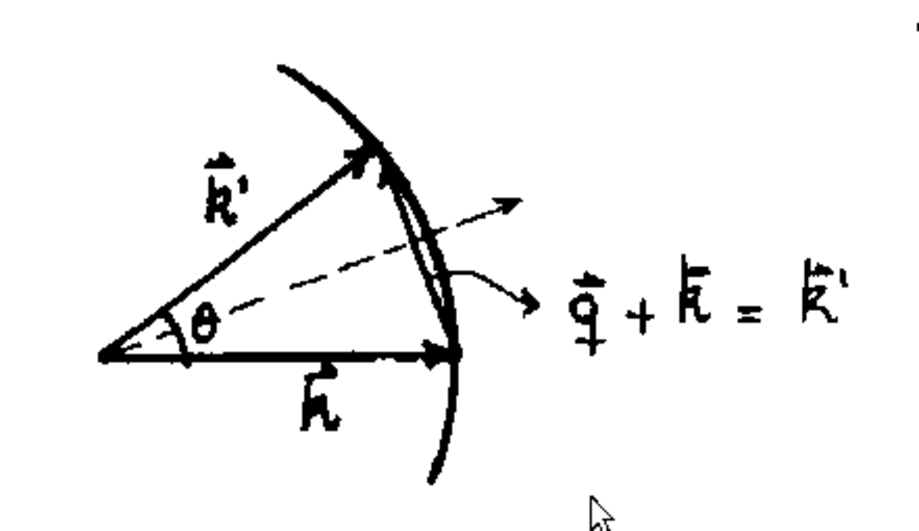
\includegraphics[width=0.5\textwidth]{images/teo2_31.pdf}
	\end{center}
	\caption{}
\end{figure} 
la transformada de Fourier del potencial es, amén de constantes, la amplitud a primer orden 
\[
	|\vb{k} - \vb{k}'| = 2k\sin(\theta/2) \qquad \text{con} \; k=k' 
\]
Entonces para cualquier potencial esféricamente simétrico se puede hacer la integral 
\[
	\dtot{\sigma}{\Omega} =
	\left|\left( \frac{2m}{4\pi\hbar}\right)^2 \int d^3x'\;V(x)\euler^{i(\vb{x}-\vb{x}')\cdot\vb{x}'}\right|^2
\]
y expresamos todo en función de $q=q(\theta)$
\[
	\dtot{\sigma}{\Omega} =
	\left| -\frac{2m}{\hbar^2} \frac{1}{q} \int_0^\infty rV(r)\sin(q) dr \right|^2
\]

Utilizando un potencial de Yukawa primero y tomando el límite para llegar al de Coulomb tenemos la sección 
eficaz de Rutherford 
\[
	\dtot{\sigma}{\Omega} = \frac{2m^2e^4}{\hbar^4}\frac{1}{16k^4\sin^4(\theta/2)}
\]

hay que tomar el potencial de Yukawa y luego el límite porque el de Coulomb diverge de entrada



% \bibliographystyle{CBFT-apa-good}	% (uses file "apa-good.bst")
% \bibliography{CBFT.Referencias} % La base de datos bibliográfica

\end{document}
